\subsection{HDBSCAN}
\label{sec:ctm-hdb}

The third and last clustering algorithm we experimented with was HDBSCAN (Hierarchical Density-Based Spatial Clustering of Applications with Noise) \cite{McInnes2017}. Similar to the previous two algorithms, it tries to group unlabeled data points with its own set of criteria. As its name implies, it tries to group points based on spatial density to ensure the resulting groups meet some density parameter.

The advantage of HDBSCAN is that it does not require us to specify the number of clusters we want to find. Instead, we specify the minimum number of points in each cluster $P$ and the algorithm will dynamically group points such that the resulting clusters have at least $P$ points. This gives us more flexibility in our parameters because choosing the number of clusters is harder than choosing the minimum number of points per cluster. We do not know the proper the number of clusters and thus must estimate it through an ad-hoc procedure. However, we do have a stronger conceptual understanding of the number of points per cluster: since we know there are only a limited number of approaches to solve an assignment and we know the majority of the students will follow similar approaches, either through collaboration or coincidence due to limited unique approaches, we know the $P$ value must be a significant fraction of the total number of students.

However, the disadvantage of this algorithm is that it is not guaranteed to be able to label every point; outlier points that cannot satisfy the group's density criteria are discarded as noise. The higher the minimum cluster size parameter $P$, the more points will be unlabeled. Ideally we want our groups to be as dense as possible so that we know the grouped points are extremely similar to each other. Ultimately, it is a balance between how many points we can label (automation rate) and how dense the resulting groups are.

Figure~\ref{fig:ctm-hdb} shows how the algorithm labels our data set based on varying minimum cluster sizes. A cluster size of 5 is able to achieve 3 groups, which is close to the 4 groups set for the previous two algorithms. However as we can see from the graph, the 3 groups are slightly sparse. As a result, we chose $P=10$ because it is able to label most of the points without sacrificing too much density; at higher cluster sizes, we do not seem to significantly increase our groups' densities.

Once we were satisfied with our parameters, we ran the HDBSCAN algorithm and designated each student's score to be equal to the \textquote{strength} of the student's corresponding group prediction returned from the algorithm.

\begin{figure}
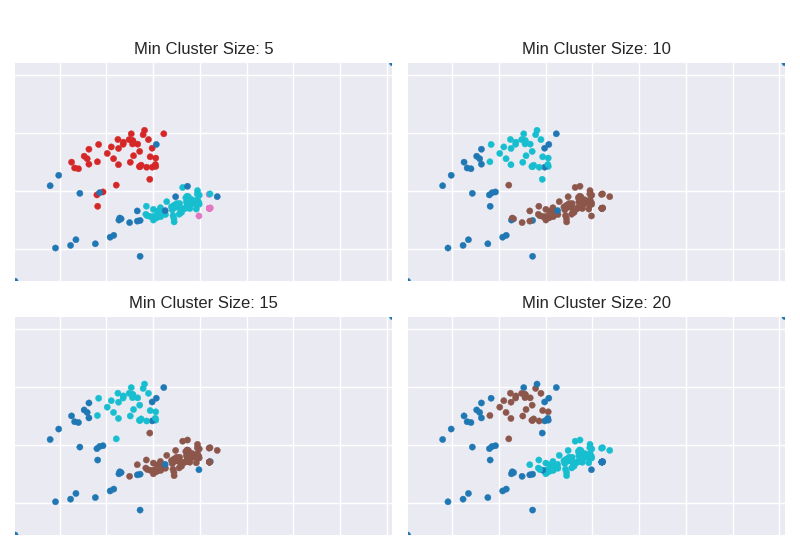
\includegraphics[width=\textwidth]{conversion-to-mark/marking_paster_nbio_ece459-a1-w2017_hdb}
\caption[HDBSCAN Clustering]{These graphs show our data points clustered with HDBSCAN using different minimum cluster size parameters. The higher the minimum size, the denser the resulting clusters. Furthermore, higher cluster sizes also result in more outlier points marked as noise (dark blue) as well as fewer total clusters. Cluster size of 5 has three different groups whereas cluster sizes of 10 and higher only have two different groups.}
\label{fig:ctm-hdb}
\end{figure}
